\chapter{Badanie projektu historycznego}
\label{chapter:verify}

Motywacją do powstania pracy była potrzeba usprawnienia procesu weryfikacji prac studentów dla zespołowego projektu informatycznego.
W ramach pracy dokonano próby oceny poprawności działania programów studentów utworzonych w ramach przedmiotu ”Podstawy Programowania” w semestrze zima 2018.
W tym celu przeanalizowano zadanie projektowe i dostępne aplikacje studenckie.
Następnie uruchomiono programy studentów lokalnie.
Ostatnim krokiem badania projektu historycznego była próba uruchomienia dostępnych aplikacji studenckich na platformie.

W rozdziale \ref{analysis_students_projects} została opisana analiza zadania i historycznych aplikacji studenckich.
Kolejna sekcja omawia lokalne uruchomienie programów, rezultaty ich działania i~napotkane problemy.
W rozdziale \ref{veryfication_platform} została opisana próba uruchomienia programów na platformie.
Ostatni rozdział zawiera podsumowanie badania historycznego projektu.

\section{Analiza zadania projektowego}
\label{analysis_students_projects}

Do zbadania rezultatów pracy studentów dla zespołowego projektu informatycznego posłużono się kodem napisanym w ramach przedmiotu podstawy programowania.
Zadaniem studentów było napisanie programu odzwierciedlającego logikę gry planszowej ”Hey, that’s mine fish”.
Aplikacja miała umożliwiać interaktywny oraz automatyczny rodzaj rozgrywki.
Zadaniem programów było wczytanie wejściowego układu planszy z~pliku, wykonanie zadanej akcji oraz zapisanie zmodyfikowanego układu planszy do pliku.
Format pliku jest jednoznacznie określony w~treści zadania i składa się z:
\begin{itemize}
    \item \textit{Wiersz 1}: \textit{m n} - dwóch wartości liczbowych oznaczających rozmiar planszy.
    \item \textit{Wiersze od 2 do m+1}: \textit{n} pól odseparowanych znakiem spacji, każde z pól jest definiowane przez dwie cyfry.
    Pierwszą oznaczającą liczbę ryb na danym polu (od 0 do 3) oraz druga będącą identyfikatorem gracza znajdującego się obecnie na tym polu (od 1 do 9 lub 0 jeśli pole nie jest zajęte).
    \item \textit{Wiersze od m+2}: trzech pól, reprezentujących kolejno: nazwę gracza (String), identyfikator gracza (od 1 do 9), liczbę punktów uzyskanych przez gracza.
\end{itemize}

Zgodnie z założeniami programy mają przyjmować następujące parametry:
\begin{itemize}
    \item \textit{phase=phase\_mark}, parametr \textit{phase\_mark} może przyjąć jedną z dwóch wartości: \textit{placement} (rozmieszczanie) lub \textit{movement} (ruch).
    \item \textit{penguins=N}, gdzie \textit{N} oznacza liczbę pingwinów (pionków) dostępnych dla każdego z graczy.
    Parametr jest używany tylko w fazie rozmieszczania.
    \item \textit{inputboardfile}, nazwa pliku wejściowego z układem planszy.
    \item \textit{outputboardfile}, nazwa pliku wyjściowego z układem planszy.
    \item \textit{id}, w przypadku podania argumentu \textit{id} program powinien wypisać identyfikator gracza i zakończyć działanie.
\end{itemize}
Pełna definicja zadania projektowego znajduje się w załączniku.

Aplikację rozwiązującą opisane wyżej zadanie można uruchomić na platformie i sprawdzić jej działanie.
Jednak przy założonych parametrach wykonania trudno jest napisać testy akceptacyjne, które pozwolą na automatyczną weryfikację programów.
Do otrzymania korzyści z użytkowania platformy należałoby zmienić założenia co do komend i~przyjmowanych parametrów, tak aby można było napisać odpowiednie i~proste przypadki testowe.
Przykładowo dla fazy ruchu wystarczyłoby dodać dwa parametry wykonania: położenie pingwina, którym chcemy poruszyć oraz docelowe miejsce, w które chcemy go przesunąć.
Faza rozmieszczania również wymagałaby modyfikacji.

W celu zbadania rezultatów projektów studenckich przeanalizowano siedem udostępnionych repozytoriów używanych przez studentów i zamieszczonych na platformie GitLab.
Wstępny przegląd repozytoriów kodu pozwolił ustalić, że spośród dostępnych grup tylko cztery ukończyły zadanie projektowe.
Dwie z pozostałych grup przerwały projekt już na samym początku semestru.
Jeden z zespołów dołączył do innej grupy w trakcie trwania projektu, przez co kod z jego pracy przed przegrupowaniem nie jest analizowany.
Z powyżej przedstawionych powodów dokonano próby lokalnego uruchomiona czterech historycznych programów studenckich.

\section{Lokalne uruchomienie historycznych programów studentów}

Lokalne uruchomienie programów studentów zostało sprowadzone do następujących kroków:
\begin{itemize}
    \item Analiza repozytorium kodu historycznych programów.
    \item Kompilacja.
    \item Uruchomienie.
\end{itemize}

Podczas każdego z powyższych kroków napotkano na kilka problemów.
Te trudności zostały omówione w kolejnych podrozdziałach.

\subsection{Analiza repozytorium kodu}

Projekt był prowadzony przez cały semestr a kod studentów systematycznie wgrywany na GitLab.
Studenci nie używali tzw. ”tagowania commitów” (ciężko też od nich tego wymagać na pierwszym roku studiów).
Z tych powodów granice wykonania kolejnych etapów są zatarte i ciężko je odtworzyć.
Zakłada się więc, że kod znajdujący się na GitLab to ostateczne wersje programów, które powinny spełniać założenia projektowe i~pozwolić na uruchomienie wersji interaktywnej oraz AI.

%team 05
Trzy grupy projektowe zamieszczały swój kod bezpośrednio w repozytorium.
Jeden zespół zamieścił go w tzn. ”snippetach” co utrudniło odszukanie i pobranie go w celu lokalnego uruchomienia.

Kolejnym problemem jest określenie wewnątrz repozytorium, która wersja kodu jest ostateczna i powinna zostać zweryfikowana.
W tym przypadku można posłużyć się datą ostatniego tzw. ”commita”, jednak nie zawsze wydaje się to być odpowiednim rozwiązaniem.
Często zdarza się, że studenci tuż przed końcem projektu (zwłaszcza na samym początku studiów) dokonują modyfikacji w swoich programach.
Takie działania bardzo często doprowadzają do powstawania dodatkowych błędów i powrotu do poprzedniej wersji rozwiązania.
%team 05
W repozytoriach istnieje wiele folderów zawierających nazwy \textit{final} przykładowo: \textit{Penguins\_final\_code}, \textit{Penguins\_final\_edition\_2}, \textit{Penguins\_final\_edition\_3}.
%team 05 i team 02

Innym problemem jest fakt, że programy dla połowy zespołów były zamieszczane w~repozytorium w postaci archiwum.
W takim przypadku śledzenie zmian w kodzie przy pomocy systemu kontroli wersji jest bardzo utrudnione.

\subsection{Kompilacja}

Kompilacja programów sprowadzała się do indywidualnego przejrzenia kodu każdego z projektów.
%team 04
Spośród wszystkich czterech projektów tylko jeden miał zdefiniowany, zawarty w repozytorium i poprawny plik Makefile.
Trzy pozostałe projekty wymagały własnoręcznej kompilacji.
Spośród nich dwie kompilacje były stosunkowo proste i zakończyły się sukcesem.
Jeden z programów posiadał pojedynczy plik z właściwym kodem aplikacja (rozszerzenie .c) a kompilacja drugiego programu sprowadziła się do skompilowania wszystkich plików w folderze.

%team 02
Dla jednego z zespołów własnoręczna kompilacja finalnej wersji aplikacji nie powiodła się.
Udało się za to uruchomić plik wykonywalny znajdujący się w jednym z podkatalogów.
Aplikacja działała jednak niewłaściwie (próba ustawienia pingwina wypisywała komunikat o poprawnym umieszczeniu na ekran, jednak plansza nie była aktualizowana) co doprowadziło do wniosku, że nie jest ona ostateczną wersją programu.
Dla tego zespołu pozyskano finalny kod programu razem z Makefile bezpośrednio od prowadzącego projekt.
Kompilacja tej wersji przebiegła pomyślnie.
Warto jednak zaznaczyć, że uzyskana wersja kodu nie była dostępna przez repozytorium GitLab.

\subsection{Uruchomienie}

Lokalne uruchomienie i ocena sposobu działania programów wymagała również indywidualnego podejścia do każdego z zespołów.
Można założyć, że w celu oceny działania programów każdy z nich zostanie uruchomiony w trybie interaktywnym.
Następnie dla każdego wykonane zostaną identyczne kroki a na koniec zostaną porównane otrzymane wyniki.

%team 02 i team 04
Dwa z programów uruchomionych w trybie interaktywnym pozwalały na wprowadzenie ruchu gracza i przeprowadzenie założonych testów.
Warto zaznaczyć, że dla jedengo z~testowanych programów bardzo szybko można było zauważyć, że logika zaimplementowana dla fazy rozmieszczania i ruchu pingwinów została napisana przez dwie różne osoby.
Dla fazy rozmieszczania współrzędne na planszy należało podać jako parę (x, y), natomiast dla fazy ruchu przyjmowane one były w postaci (y, x).

Jeden z programów uruchomiony w trybie interaktywnym nie pozwalał na umieszczenie pingwina na planszy i nie zapisywał wyniku do pliku wynikowego.
Wyświetlana przez program plansza była nieprawidłowa i nie pozwalała na poprawne sparsowanie.
Warto dodać, że dla tego programu przejście pomiędzy trybem AI a interaktywnym wymagało zmiany stałej w jednym z plików zawierających kod programu oraz ponownej kompilacji.

Jeden z programów uruchomił się w wersji automatycznej rozgrywki.
Sprawia to, że przetestowanie dla założonego wcześniej schematu jest niemożliwe, ponieważ w tym trybie nie mamy wpływu na ruch pingwinów.
Dodatkowo nie da się przez to ocenić, jak zachowuje się program dla przypadków brzegowych, ponieważ nie ma możliwości ustawienia pingwinów w dowolnej lokalizacji.
W tym przypadku ocena sposobu działania programu mogłaby opierać się na przeanalizowaniu algorytmu AI zaimplementowanego przez studentów i porównaniu jego działania z wynikiem symulacji.
Ze względu na brak dokumentacji dotyczącej działania algorytmu AI pominięto ocenę sposobu działania tego programu.

\section{Uruchomienie programów na platformie}
\label{veryfication_platform}

Początkowym założeniem dla uruchomienia programów na platformie było utworzenie pojedynczego projektu oraz czterech grup projektowych dla każdego z badanych projektów historycznych.
Dla projektu planowano utworzyć dwa etapy: \textit{placement} i \textit{movement} wraz z przypadkami testowymi.
Jednak już podczas analizy i lokalnego uruchamienia programów okazało się, że utworzenie wartościowych testów akceptacyjnych dla projektu historycznego nie będzie możliwe.
Wynika to między innymi z tego, że programy działają w trybie interaktywnym, czekając na reakcję użytkownika, której nie można zasymulować przy użyciu aktualnej wersji platformy.
W przypadku trybu AI nie jest udokumentowane, w jaki sposób powinny zachować się programy, stąd napisanie testów akceptacyjnych dla tego trybu jest również bezcelowe.

Z powyższych powodów uznano, że historyczne programy zostaną uruchomione przy pomocy narzędzia, jednak poprawność ich wykonania nie będzie oceniana poprzez testy akceptacyjne.
W ramach platformy oceniono samą możliwość uruchomienia programów przy jej użyciu.
W tym celu porównano otrzymane na platformie logi z wynikiem lokalnego uruchomiania aplikacji.
W przypadku, gdy programy nie zalogowały błędów wykonania i wypisały takie same logi, jak w lokalnej konsoli uznane zostało, że uruchamiają się poprawnie na platformie.

W początkowym podejściu w wyniku analizy działania uruchomionych lokalnie programów zdecydowano się na utworzenie jednego projektu i zdefiniowanie czterech różnych etapów (oddzielnych dla każdego z programów).
Ze względu na podawane parametry w~postaci argumentów do programu plik Dockerfile dla tego projektu wyglądał następująco:

{\fontfamily{qcr}\selectfont
\tiny
\begin{lstlisting}

    FROM gcc:4.9

    CMD ["./home/app", "phase=placement", "penguins=2", "/home/input.txt", "/home/output.txt"]

\end{lstlisting}
}

Definicja projektu na platformie dla widoku podglądu prowadzącego została przedstawiona na rysunku \ref{fig:veryfication_first_project}.

\begin{figure}[h]
    \centering
    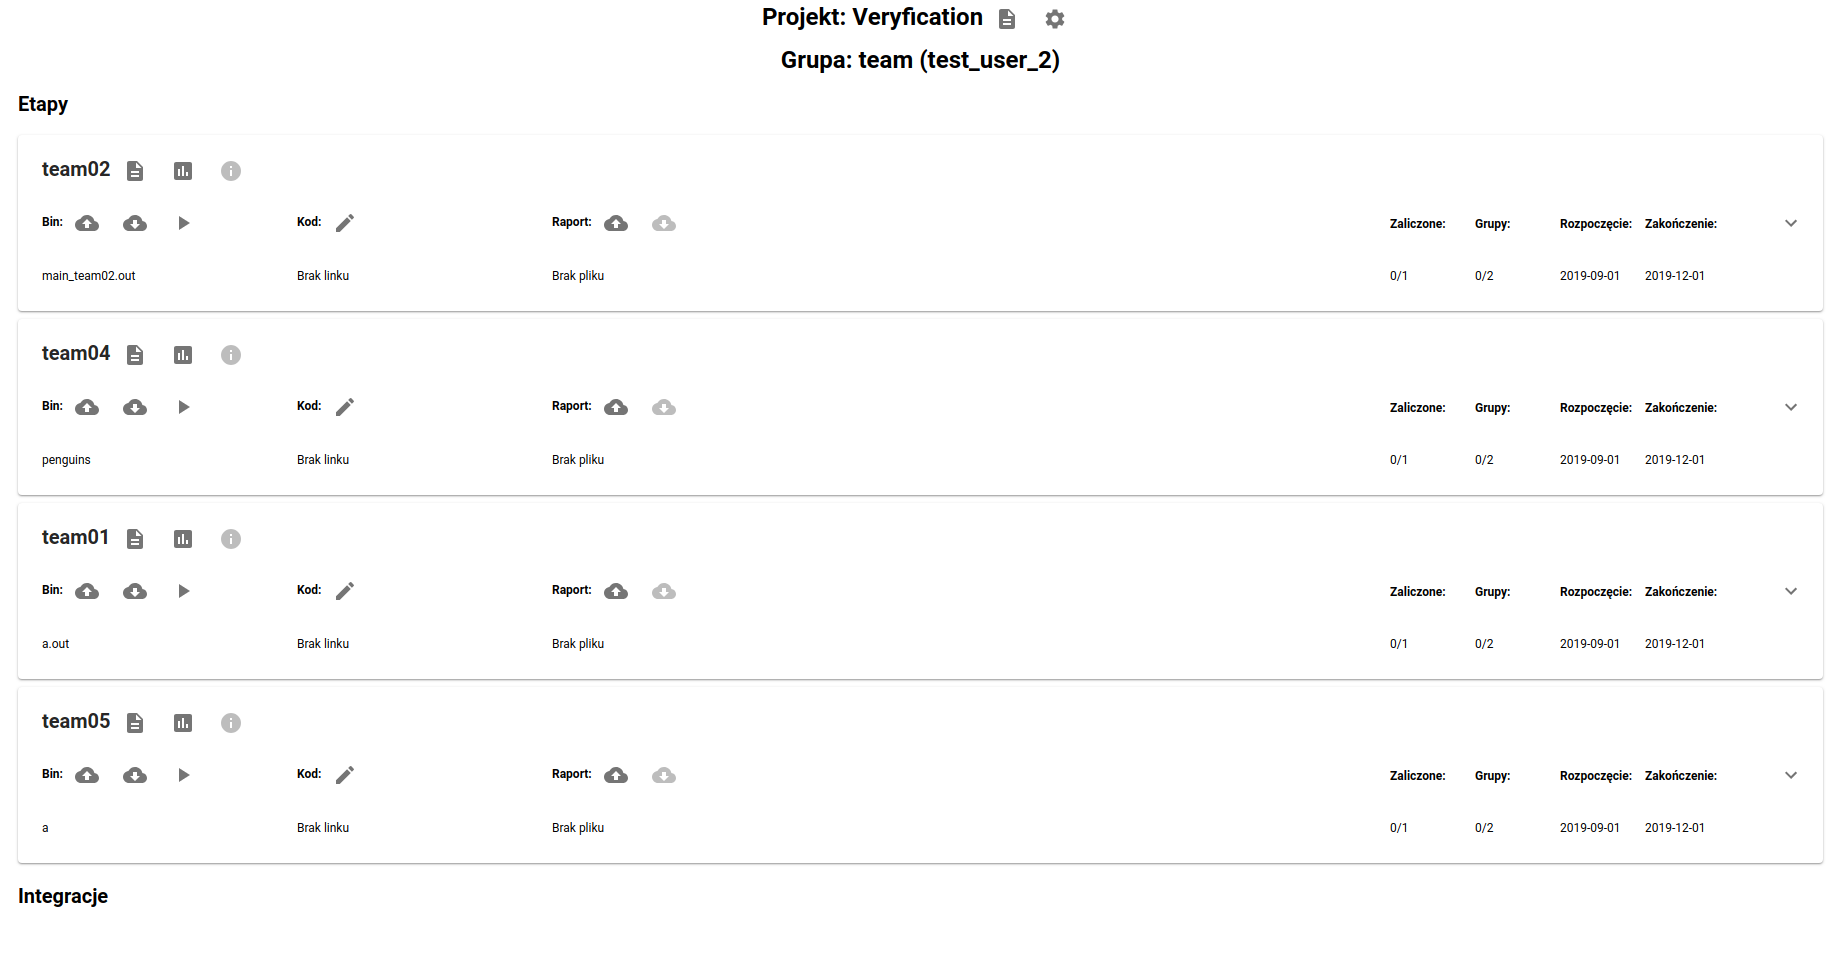
\includegraphics[width = 12cm]{chapter06/veryfication_first_project.png}
    \caption{Projekt dla weryfikacji platformy przy pomocy historycznych programów studentów (źródło własne).}
    \label{fig:veryfication_first_project}
\end{figure}

Dla każdego z czterech etapów (reprezentujących historyczne programy studentów) utworzono prosty przypadek testowy, gdzie jako \textit{input} i \textit{output} wprowadzono plik z planszą.
Został on wybrany losowo spośród zawartych w repozytoriach historycznych grup testowych plików wejściowych.
Następnie uruchomiono wszystkie cztery etapy.
Po przejrzeniu logów okazało się, że tylko jeden program uruchomił się poprawnie (załączony dla etapu \textit{team05}).
Była to aplikacja z tego samego repozytorium, z którego załączono plik z planszą dla przypadków testowych.
Inne dwa programy (etapy \textit{team02} oraz \textit{team04}) nie wypisały logów, natomiast jeden wypisał komunikat o niepoprawnym formacie pliku wejściowego (\textit{team01}).

Dla programu dołączonego do etapu \textit{team01} zmieniono plik wejściowy i wejściowy na taki, który znajdowały się w repozytorium razem z tym programem.
Aplikacja została następnie uruchomiona i wyniku swojego działania wypisała logi.

Programy załączone do etapów \textit{team02} oraz \textit{team04} zostały ponownie przeanalizowane poprzez lokalne uruchomienie.
W wyniku tego okazało się, że uruchamiają się one w wersji interaktywnej bez podawania argumentów wykonania.
Aby uzyskać informację zwrotną z ich działania utworzono nowy projekt z poniższą definicją środowiska:

{\fontfamily{qcr}\selectfont
\tiny
\begin{lstlisting}

    FROM gcc:4.9

    CMD ["./home/app"]

\end{lstlisting}
}

W ramach projektu zostały utworzone dwa etapy:  \textit{team02} oraz \textit{team04}.
Następnie załączono i uruchomiono aplikacje.
Program załączony do etapu \textit{team02} uruchomił się w wersji interaktywnej i wypisał logi.

Aplikacja dla etapu \textit{team04} po raz kolejny nie zostawiła informacji zwrotnej z wyniku wywołania.
W celu rozwiązania problemu przeanalizowano część kodu aplikacji.
Ustalono, że problem może wynikać z pętli \textit{while}, która czeka na pobranie znaku od użytkownika.
Po usunięciu jej z kodu programu, rekompilacji i ponownym uruchomieniu programu na platformie uzyskano logi z wykonania aplikacji.


\section{Podsumowanie}
\label{verification_summary}

Lokalne uruchomienie historycznych programów pokazuje, że proces weryfikacji pracy studentów jest trudnym i czasochłonnym zadaniem.
Podejście do każdego z zespołów jest indywidualne na każdym z kroków: analiza kodu, kompilacja, uruchomienie i ocenia działania.

Ustalenie ostatecznej wersji kodu pomimo załączania go do systemu kontroli wersji jest problematyczne.
Aby mieć pewność co do tego, który wariant jest ostateczny wymagana jest konsultacji ze studentami.

Budowanie aplikacji jest utrudnione.
Studenci nie załączają skryptów do budowy programów, przez co proces wymaga dodatkowej analizy kodu.

Sama ocena aplikacji jest w pełni indywidualnym procesem dla każdej z grup.
Problemem nie jest tylko różny wygląd interaktywnych interfejsów oraz format przyjmowanych wewnątrz nich danych.
Okazuje się, że programy nie przestrzegają zdefiniowanych założen projektowych co do przyjmowanych parametrów i formatu planszy.
Aplikacje przyjmują inne parametry wejściowe i w różny sposób definiują położenie na planszy.
Widać to między innymi na przykładzie ustalania pozycji pingwina.
Podczas badania programów spotkano trzy różne sposoby ustalania położenia identyfikowane przez podanie: dwóch liter, litery i cyfry oraz dwóch cyfr.
Nawet w przypadku jednego programu wewnętrzny format przyjmowanych parametrów położenia (x, y lub y, x) może być zupełnie inny w~zależności od wykonywanej fazy.
Prowadzący projekt mają bardzo trudne zadanie podczas oceny efektów pracy zespołów, ponieważ pomimo przyjętych takich samych założeń projektowych rezultat działania każdej z aplikacji jest inny.

W przypadku przyjmowanych różnych formatów planszy i parametrów integracja programów jest praktycznie niemożliwa.
Opisane powyżej komplikacje mogą wystąpić podczas sprawdzania każdego z etapów i nałożyć się w momencie próby przeprowadzenia integracji programów.

Uruchomienie aplikacji i testowanie ich w trybie interaktywnym znacznie utrudnia ocenę ich działania.
Wymaga ona prześledzenia ruchu pingwinów na wypisywanej na konsoli planszy.
Część informacji nie mieści się na jednym oknie terminala i jest ucinana.
Dodatkowo większość aplikacji nie wypisuje informacji zwrotnych z komunikatem o błędzie, stąd ciężko ocenić czy zadana komenda wykonała się poprawnie.

W przypadku trybu AI ocena programów jest jeszcze trudniejsza.
W raportach brakuje dokumentacji co do tego, jak aplikacja będzie zachowywać się dla tego wariantu rozgrywki.
Ocenę programów można byłoby oprzeć na przeprowadzeniu opisanego w~treści projektu turnieju.
Przeprowadzenie wspomnianych zawodów sprowadza się jednak do przeprowadzenia integracji aplikacji, co jak zostało opisane wcześniej, nie jest możliwe dla historycznych programów.

Te wszystkie powyższe problemy sprawiają, że właściwa ocena programów z perspektywy czasu i bez kontaktu ze studentami jest praktycznie niemożliwa.
Aplikacje można ocenić pod względem estetycznym.
Można również uznać za niespełniające pełnych założeń te programy, które nie pozwalają na przeprowadzenie rozgrywki w trybie interaktywnym.
Nawet w przypadku programów pozwalających na interaktywną rozgrywkę przetestowanie przypadków brzegowych jest czasochłonnym i indywidualnym zadaniem.
Szczegółowa ocena działania aplikacji wymagałaby wniknięcia do kodu programów, co jest bardzo trudnym zadaniem.
Zwłaszcza w przypadku kodu pisanego przez studentów pierwszego roku studiów, którzy nie znają jeszcze dobrych praktyk programistycznych.

Zbadanie projektu historycznego potwierdziło potrzebę wprowadzenia narzędzia, które usprawni proces weryfikacji pracy studentów.
Dzięki platformie można wyeliminować indywidualne podejście do każdej z grup projektowych i zmniejszyć czasochłonność oceny poszczególnych etapów.
Pozwoliłaby ona na jednoznaczną ocenę logiki działania każdej z aplikacji na podstawie uruchomienia zestawu testów integracyjnych.
Co więcej, dzięki webowemu interfejsowi możliwe byłoby porównanie postępów w~ramach projektów w~przypadku realizacji dla dwóch różnych semestrów.
Mogłaby to być przydatna informacja dla prowadzącego.

Wszystkie lokalnie uruchomione historyczne programy studenckie udało się uruchomić na platformie uzyskując przy tym informację zwrotną w postaci logów.
Oznacza to, że platforma pozwala na zestawienie środowiska potrzebnego do przeprowadzenia studenckiego projektu informatycznego.
Łatwo jednak zauważyć, że użycie platformy do przetestowania historycznych programów nie przynosi wiele korzyści.
Wynika to ze sposobu definicji założeń projektowych, które nie uwzględniały użycia narzędzia do weryfikacji pracy studentów.
Aby wykorzystać w pełni potencjał platformy należałoby zmienić historyczną koncepcję zadania, tak aby aplikacje przyjmowały argumenty wykonania z~pliku zawierającego parametry.
Warto zaznaczyć, że modyfikacje nie oznaczają wykluczenia wersji interaktywnej oraz AI.
Programy studenckie dalej mogą używać tych dwóch trybów pracy (choć nie muszą).
Rozszerzenie założeń o przyjmowanie parametrów z pliku pozwoliłoby na przetestowanie głównej logiki programów i byłoby pomocne przy ocenie działania aplikacji.

Przy niewielkiej modyfikacji zadania, można osiągnąć dużo lepszą automatyzację procesu oceny efektów pracy zespołów.
W kolejnym rozdziale zostaną omówione zmiany założeń zadania historycznego, tak aby osiągnąć korzyści wynikające z korzystania z platformy.
Opisane również zostaną wnioski z przeprowadzenia symulacji zmodyfikowanego projektu historycznego na testowej grupie absolwentów.




